\documentclass[oneside]{article}
\usepackage{fullpage}
\usepackage[small]{titlesec}
\usepackage[pdftex]{graphicx}
\usepackage[round,sectionbib]{natbib}
\bibliographystyle{plainnat}
\DeclareGraphicsExtensions{.png,.pdf}
\graphicspath{{examples/}}
\usepackage{hyperref}
% \usepackage{setspace} 
% \doublespacing

\begin{document}
\title{Two techniques for teaching inference: the statistical justice system and visual inference}
% Inference without mathematics
% Revealing the power of inference without maths
% A new machinery for teaching inference that focuses on the concepts
% Inference from real life
% Sesame street simple inference
\author{Hadley Wickham, Heike Hofmann, Dianne Cook, Andreas Buja}
\date{13 May 2010}

\maketitle
\begin{abstract}

The statistical justice system makes hypothesis testing easier to understand and remember by connecting it to a concrete and familiar entity: the criminal justice system.

\end{abstract}

\section{Introduction}

Inference, testing and estimation, is one the most important aspects of statistics, yet it is one that students struggle to understand. This paper introduces two techniques that we have found helpful to give students metaphors to better understand how it works. 

This short note introduces the statistical justice system ({\sc sjs}), a fun and memorable metaphor for teaching hypothesis testing based on its similarity to the criminal justice system. Hypothesis testing is an important part of statistics, but students often struggle because of it is abstract and has convoluted terminology (e.g. fail to reject the null). The statistical justice system provides a concrete and familiar metaphor on which to pin new terminology. The idea of connecting hypothesis testing to the justice system is not new (wikipedia even mentions parts of it in the article on hypothesis testing), but we have not been able to find a published account that goes into complete detail.

Visual inference \citep{buja:2009,me:inf4info} is a rigorous alternative to classical inference, that uses the same principles, apart from two aspects: the test statistic, and the mechanism of computing similarity. The test statistic is now a plot of the data, and instead of a mathematical measurement of difference, we use a human judge, or even jury. Compared to graphics alone, visual inference offers a rigorous approach to avoid seeing pattern in noise,  and compared to purely mathematical inference it tests a much wider set of potentially interesting hypotheses.

``Sesame street simple'', but leads to rigorous hypothesis testing. \url{http://vimeo.com/15791526}

Visual inference is useful for teaching inference because to start students just need to be able to recognise which plot is difference.  This makes concrete the ideas of the {\sc sjs} and helps students to build an understanding of what a null distribution (distribution of innocents) looks like.  We'll illustrate these ideas with a data set that has worked for us in class: shot attempts by the Los Angeles Lakers in the 2008/2009 {\sc nba} season.

\section{The statistical justice system}

A suspect (data set) is accused of a crime (having a particular parameter value) and is declared guilty or not guilty based on the results of a trial (statistical test). Each trial has a defence (advocating the null hypothesis) and a prosecution (advocating the alternative hypothesis). On the basis of how evidence (the test statistic) compares to a standard (the null distribution), the judge makes a decision to convict (reject the null) or acquit (fail to reject the null hypothesis).

In the {\sc sjs}, unlike in the criminal justice system, evidence is based on the similarity between the accused and known innocents. The population of innocents is called the null distribution and is generated by the combination of null hypothesis and test statistic. Typically, the level of guilt of the suspect is summarised with a single number, the proportion of true innocents who appear more guilty than they do. This is the $p$-value, the probability that a truly innocent person would look as (or more) guilty than suspect.  (We particularly like the description of the $p$-value in this metaphor - it's concrete and easy to understand.)

There are two types of mistakes we can make in our decision: we can falsely acquit a guilty dataset (a type II error, or false negative), or falsely convict an innocent dataset (a type I error, or false positive). Just as in the criminal justice system, the costs of these two mistakes are not equal and vary based on the severity of the consequences (the risk of letting a guilty shoplifter go free is not equal to the risk of letting a guilty axe-murderer go free). 

As in the criminal justice system, we can never prove that a suspect is innocent (absence of evidence is not evidence of absence). This is why a suspect is innocent until proven guilty, and why we fail to reject the null rather than accepting the alternative.

\section{Visual inference}
\label{sec:visual_inference}

Surprisingly, using our Sesame Street skills to pick ``which one of these things is not like the others'', we can generate a rigorous hypothesis test. The basic idea of visual inference is to (without looking at it first) embed the plot of the true data in a set of $n - 1$ null plots, plots of data from the null distribution. You then look at the panel of plots and pick the plot that is most unusual. If you correctly pick the true data as being different, then you have evidence ($p = 1/n$) that there is signal, and you are not just responding to random fluctuations. In this paper we use $n = 10$, giving a p-value of 0.1 if we identify the true data as being the most unusual. In situations we space isn't so limited we use $n = 20$ to so a successful identification gives the customary p-value of $0.05$.

To illustrate these ideas we'll use examples from classes that I taught, based on play-by-play data from Los Angeles Lakers games in the 2008 {\sc nba} season. 

\subsection{Poisson, exponential and gamma distributions}
\label{sub:univariate}

(There are a number of reasons we'd suspect that this distribution isn't Poisson, not least that multiple points can be scored in one instant of time, an important theme of pragmatic statistics is what is useful, and as long as the Poisson distribution is close to the true distribution it can still be useful, and is indeed used for modelling games of this nature by sports statisticians.)

Is the distribution of points scored by the Lakers a Poisson distribution? Or in more formal statistical language: do we reject or fail to reject the null hypothesis that the data comes from a Poisson distribution? In statistical justice system language: do we declare this dataset guilty or not guilty of the crime of not coming from a Poisson distribution. Figure~\ref{fig:poisson} hides the true dataset in a lineup of innocents datasets drawn from the Poisson distribution. Which plot looks the most unusual?

\begin{figure}[htbp]
  \centering
    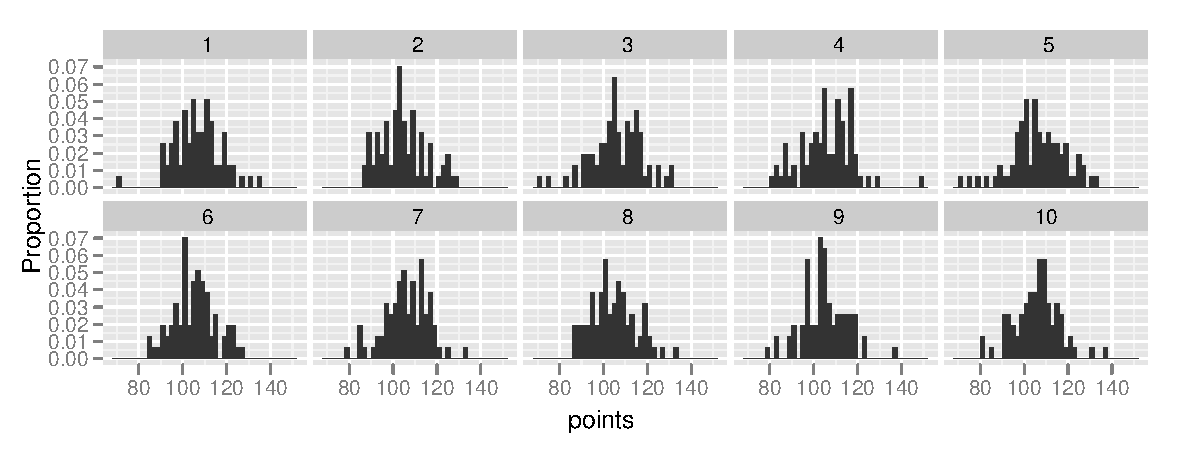
\includegraphics[width=0.9\linewidth]{poisson}
  \caption{The distribution of points scored per game by the Lakers, hidden amongst nine plots generated under the null hypothesis of a Poisson distribution.}
  \label{fig:poisson}
\end{figure}

Answer: \reflectbox{True data is in panel three}. If you identified this panel as being the most unusual, then we have some evidence to suggest that the data is not from a Poisson distribution. In this case, it does not look like we have enough evidence to convict this dataset, so we declare it not guilty.

Students may be familiar with the theoretical shape of the distribution, but few are familiar with how much this shape varies when we have a sample of the data. Seeing the null distributions is also helpful as a calibration: we hope that when students look at histograms in the future, they will remember these plots and how much the shapes varied. Mathematically testing the difference requires a lot more mathematical machinery ($\chi^2$ distribution and test, goodness of fit tests) etc, and introducing that when students are still struggling with the concept of distributions is a recipe for confusion.

% Compare this to plot that shows the data distribution overlaid with a theoretical distribution, Figure~\ref{fig:poisson-overlay}
% 
% \begin{figure}[htbp]
%   \centering
%     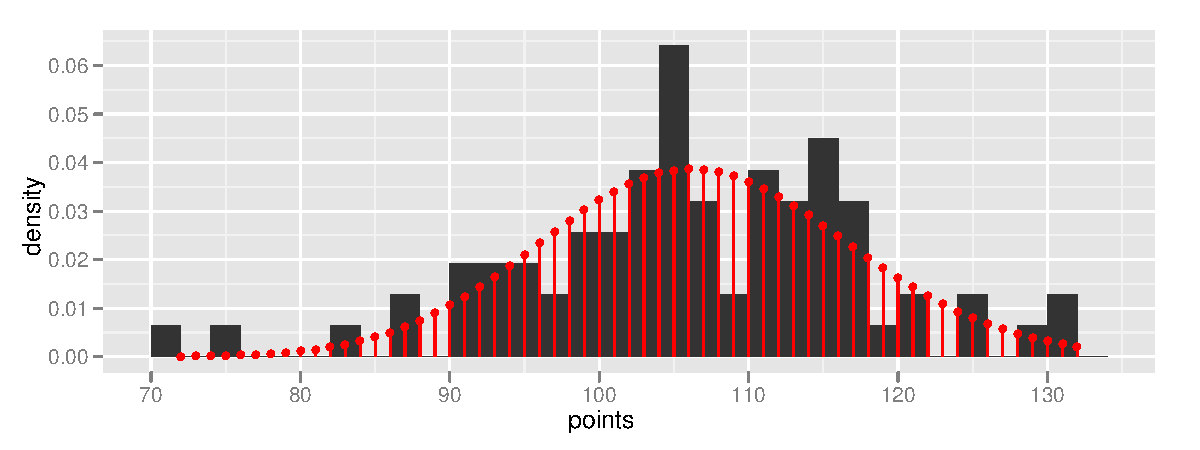
\includegraphics[width=0.5\linewidth]{poisson-overlay}
%   \caption{Data overlaid with theoretical pdf in red.}
%   \label{fig:poisson-overlay}
% \end{figure}

In prosecuting a crime, we might use forensics to dig up more evidence. In this case we can use the known relationship between the Poisson and exponential distributions: if the distribution of waiting times is exponential, then the distribution of counts in a fixed time will be Poisson. So let's look at the distribution of waiting times, how long do we wait between seeing points scored in a basketball game? Figure~\ref{fig:exponential} shows the distribution from the data hidden amongst 9 null plots generated from an exponential distribution with parameters matched to the data.

\begin{figure}[htbp]
  \centering
    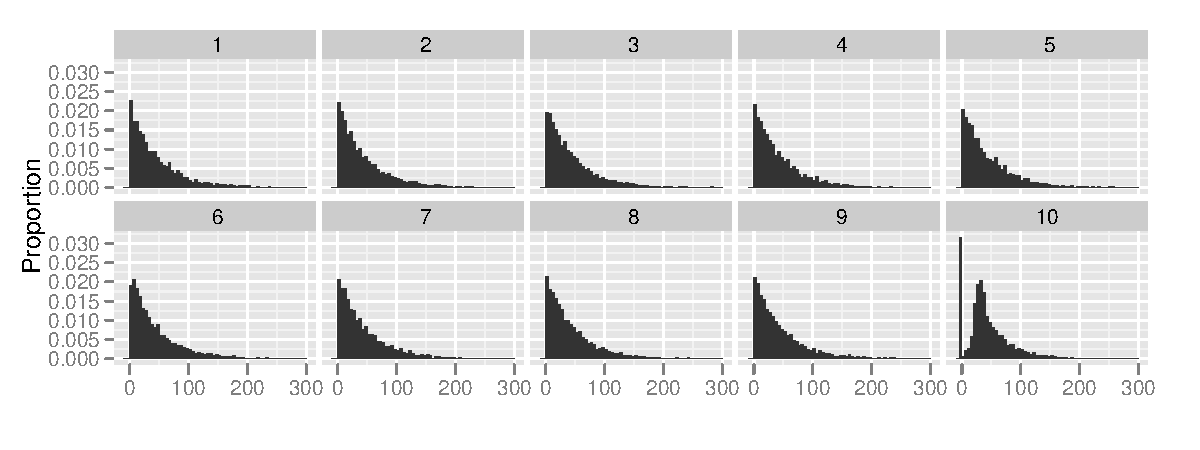
\includegraphics[width=\linewidth]{exponential}
  \caption{The distribution of waiting times between points, hidden amongst nine plots generated under the null hypothesis of a exponential distribution. X-axis truncated to maximum of 300 seconds.}
  \label{fig:exponential}
\end{figure}

The true data, \reflectbox{(in panel ten)}, is strikingly obvious: there are a large number of waiting times that are 0. These represent free throws and other penalties when the game clock is stopped. Figure~\ref{fig:gamma} removes free throws, focussing only on the waiting time between field goals, and for the null plots uses the slightly more flexible gamma distribution. Can you spot the true data?

\begin{figure}[htbp]
  \centering
    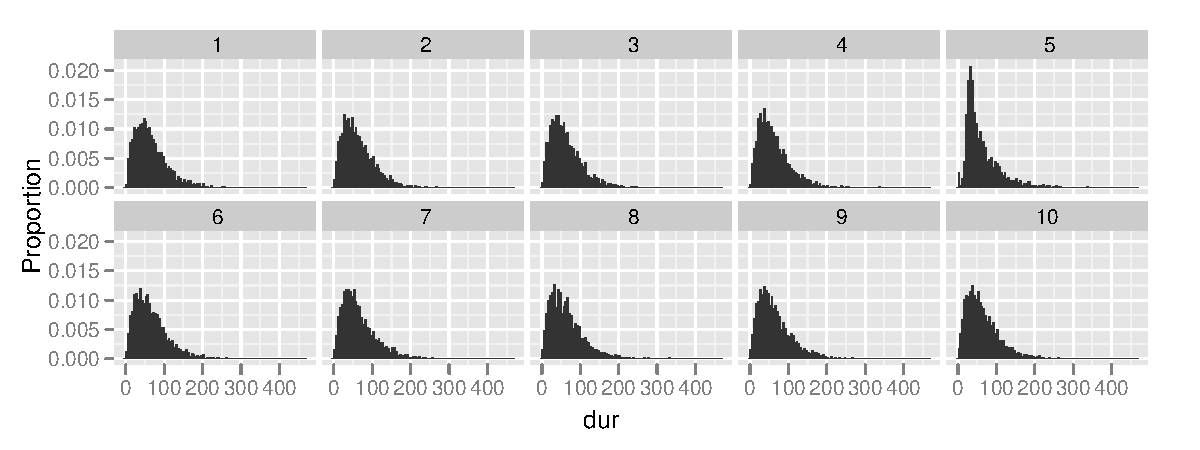
\includegraphics[width=\linewidth]{gamma}
  \caption{The distribution of waiting times between field goals, hidden amongst nine plots generated under the null hypothesis of a gamma distribution. X-axis truncated to maximum of 300 seconds.}
  \label{fig:gamma}
\end{figure}

The true data is in \reflectbox{panel five}, and again the difference is striking and we sufficient evidence to convict: the data does not come from a gamma distribution. This is unfortunate because the parameters of the gamma ($\alpha = 28$, $\beta = 2.3$) have a nice interpretation here: the average rate of shot attempts is 1 per 28 seconds, and on average, 1 in 2.3 are successful.

\subsection{Scatterplots}
\label{sub:bivariate}

Moving from time to space, 1d to 2d, intro to statistics to linear models, we will next look at the position of 3 pointer shot attempts.  Figure~\ref{fig:three-pt} shows these in both Cartesian and polar coordinates.  It looks like there is a subtle deviation from a circle: acute shots are taken closer than straight shots. Can we model this pattern with a quadratic model?

\begin{figure}[htbp]
  \centering
    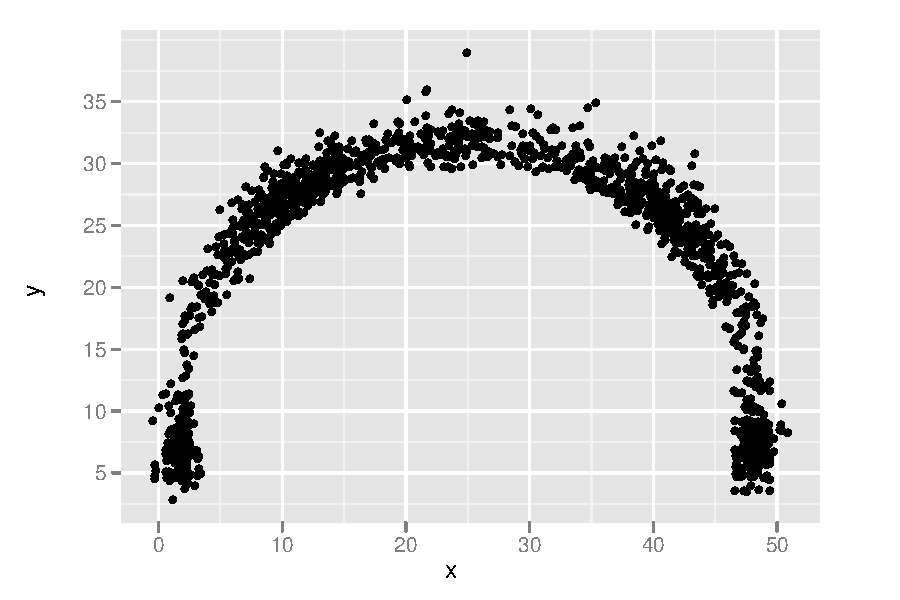
\includegraphics[height = 2in]{x-y}
    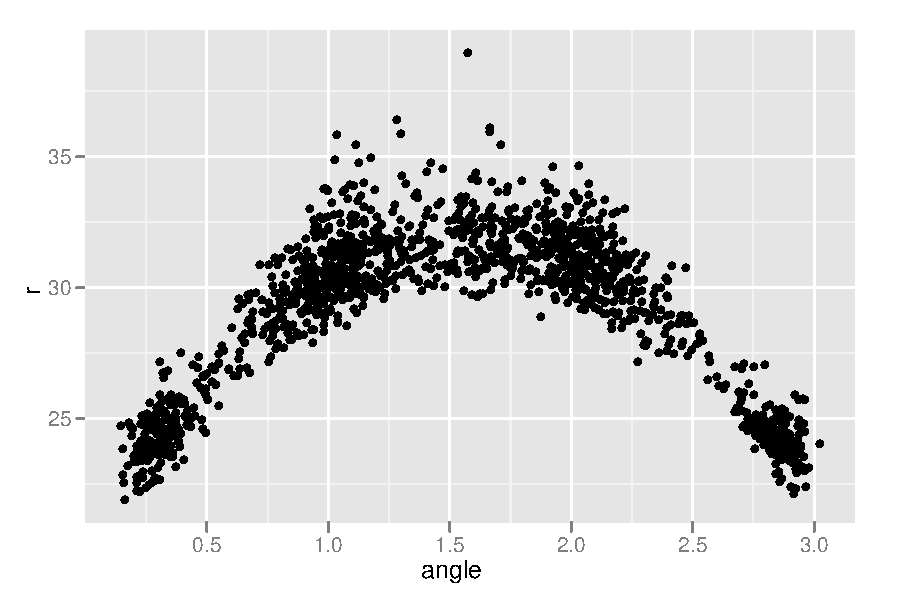
\includegraphics[height = 2in]{angle-r}
  \caption{(Left) Scatterplot of locations of three pointers. (Right) Location of three pointer attempts in polar coordinates. The steeper the angle, the shorter the distance.}
  \label{fig:three-pt}
\end{figure}

Figure~\ref{fig:quadratic} shows the true scatterplot embedded amongst nine innocent datasets generated under the null hypothesis that the data is generated by a linear model with quadratic term in angle. 

\begin{figure}[htbp]
  \centering
    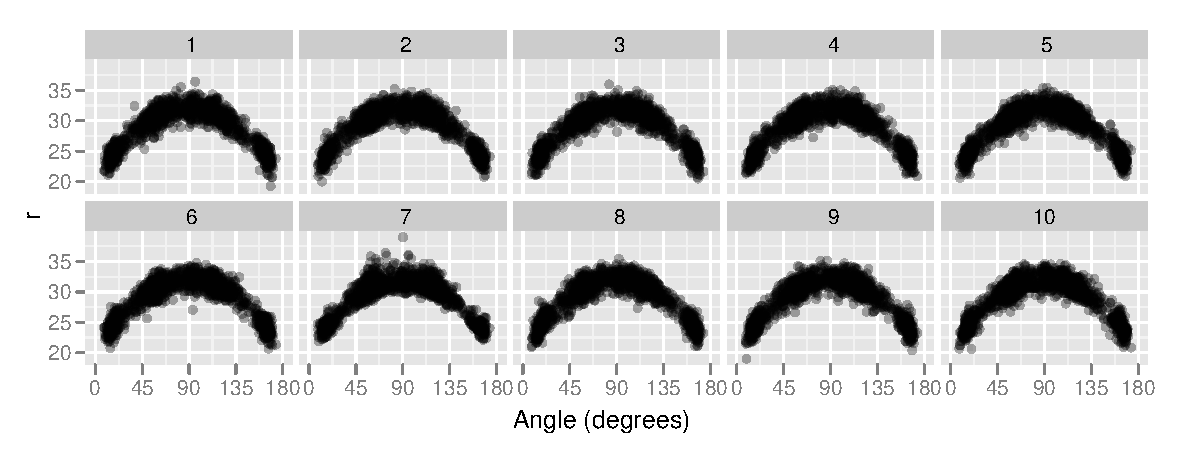
\includegraphics[width = \linewidth]{quadratic}
  \caption{One plot showing the true relationship between angle and radius embedded amongst 9 null datasets. Which plot doesn't belong?}
  \label{fig:quadratic}
\end{figure}

\section{Conclusions}

I used this presentation of hypothesis testing in class this year. Anecdotally, it seemed to help students better understand testing. The connection between the arguments of the defence and the null hypothesis helped them correctly identify the null in problems. The description of the $p$-value as the probability an innocent would look this guilty, seemed to help to avoid some of the common misinterpretations.

Students liked this presentation of the material and in the end of semester reviews, 5 out of 43 said that it was their favourite lecture of the semester. This is pretty impressive for a lecture on hypothesis testing!

In my mind, one of the most exciting possibilities of graphical inference is the way it separates the key ideas of hypothesis testing from the mathematical tools needed to support them. This makes it possible to start, on the very first day, with inference - getting to the heart of statistics on the first day of an introductory course. This is exciting because it normally has to wait to the end, once all the necessary mathematically machinery has been developed.  This 

% bibtool -x sjs.aux > references.bib
\bibliography{references}
\end{document}
